\newpage
\section{2D System Simulation}\label{sec:2d_sim}
As it is mentioned earlier, the whole idea of the project is to make the antenna of the UA and the GS point at each others. To achieve this its needed to know the angle of the antennas and their optimal angle, which is when they point exactly at each others. To be able to point the antennas towards each others two controllers will be implemented. In this section an algorithm to calculate the optimal angle for the 2D system will be introduced. Furthermore the implementation of the controllers will be explained.

\subsection{Scenario}
In Figure \ref{fig:ua_gs} it is shown a scenario where the antennas of both GS and UA change after some periods of time. In the top part of the figure it shows the angle of the UA ($\theta_{ua}$) and the optimal angle ($\theta_{opt\_ua}$) that the antenna want to be in. In the lower part of the figure it shows the angle of the GS ($\theta_{gs}$) and the optimal angle ($\theta_{opt\_gs}$). 

\begin{figure}[h]
	\centering
	
	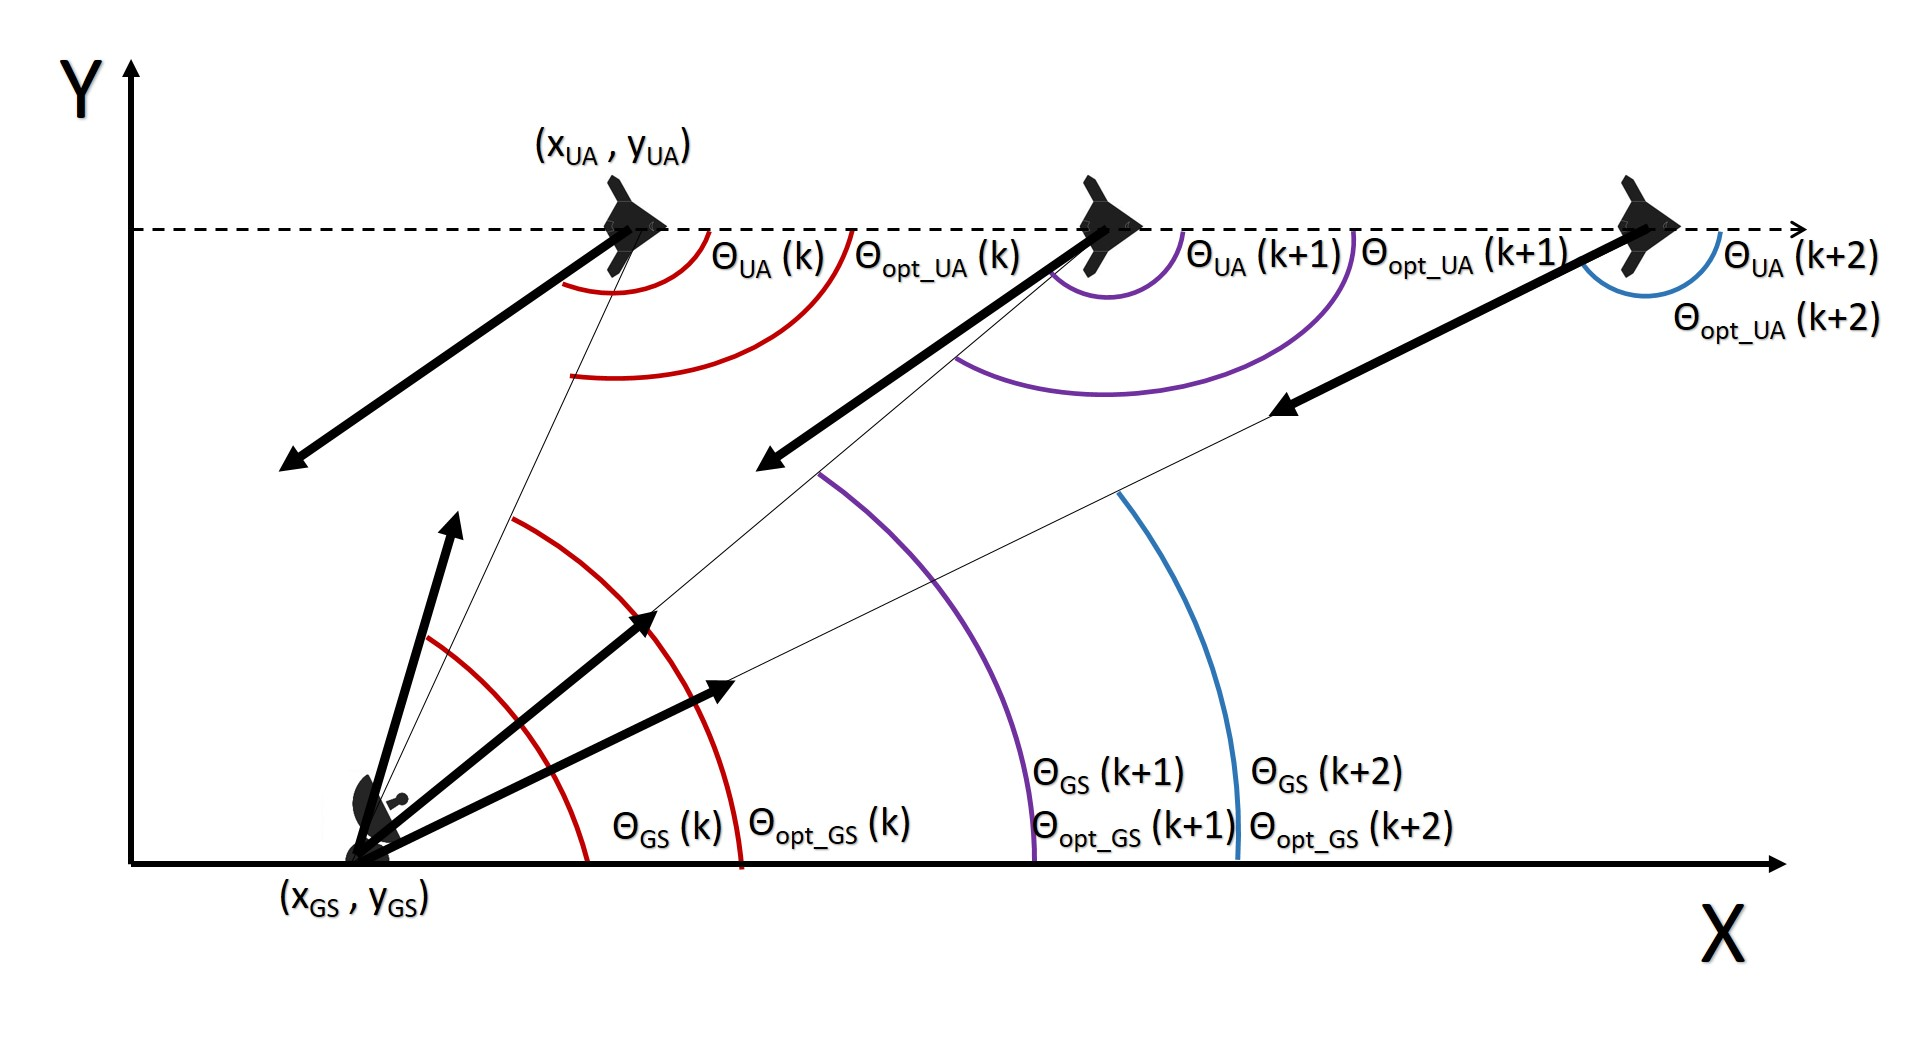
\includegraphics[scale=0.45]{figures/drone_gs_ex_1.jpg}
	\caption{Example of a GS-UA scenario}
	\label{fig:ua_gs}
\end{figure}

As it is seen on the figure at time k the antenna on the UA ($\theta_{ua} (k)$) is not equal the optimal angle ($\theta_{opt\_ua}(k)$). The same goes with the $\theta_{gs}(k)$ and the optimal angle $\theta_{opt\_gs}(k)$. As the aircraft moves further on the X-axis the angles of the GS and UA go closer to the optimal angle. 

\subsection{System overview}
The system presented have 4 inputs and 2 outputs. The system is shown in figure \ref{fig:2d_system}. 

\begin{figure}[h]
	\centering
	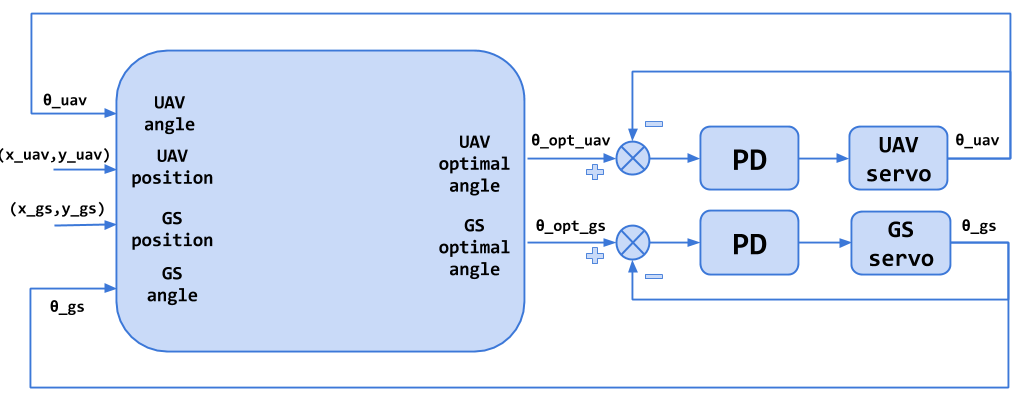
\includegraphics[scale=0.42]{figures/2d_system.png}
	\caption{2D sytem overview}
	\label{fig:2d_system}
\end{figure}
The first block of the system takes as inputs the parameters below and computes the optimal angles for the GS ($\theta\_opt\_gs$) and UAV ($\theta\_opt\_ua$) antennas, such that a strong communication link is achieved. \\

\noindent The 2 outputs, of the first block, that it is needed to control are:
\begin{itemize}
	\item UA antenna angle ($\theta_{ua}$)
	\item GS antenna angle ($\theta_{gs}$)
\end{itemize}

\noindent The system's inputs are as follows:
\begin{itemize}
	\item UA antenna angle ($\theta_{ua}$)
	\item GS antenna angle ($\theta_{gs}$)
	\item UA position ($x_{ua},y_{ua}$)
	\item GS position ($x_{gs},y_{gs}$)
\end{itemize}   

The right part of the Figure \ref{fig:2d_system} shows two PD controllers where each of them have a servomotor connected. The PD controller is explained in Section \hl{\textbf{foo}}  and the servomotor is explained in Section \hl{\textbf{foo}}. The left block have two output which is $\theta\_opt\_ua$ and $\theta\_opt\_gs$. They are the optimal angle, which is described in section \hl{\textbf{foo}}, that the UA and GS need to have to be pointing at each other (Figure \ref{fig:drone_gs}). The PD controllers purpose is to make the servomotors rotate the antenna to the correct position. The PD controllers take the error ($\theta\_opt\_ua - \theta\_ua$) for the UA and ($\theta\_opt\_gs - \theta\_gs$) for the GS, and make the servomotors rotate the antenna to the correct position. When the error is zero, which means the input to the PD controller is zero, the antennas are at the correct angles.

\subsection{Simulations}
To verify that the 2D simulations work, some simulations are made. In the first simulation the UA is simulated by starting in (0,50) and going to (100,50), which means that the aircraft is only moving in the x-axis. The simulation is shown in figure \ref{fig:gs_angle_vs_optimal} where the top one is showing the UA angle versus the optimal angle and the bottom one is showing the GS angle versus the optimal one. 

\begin{figure}[h]
	\centering
	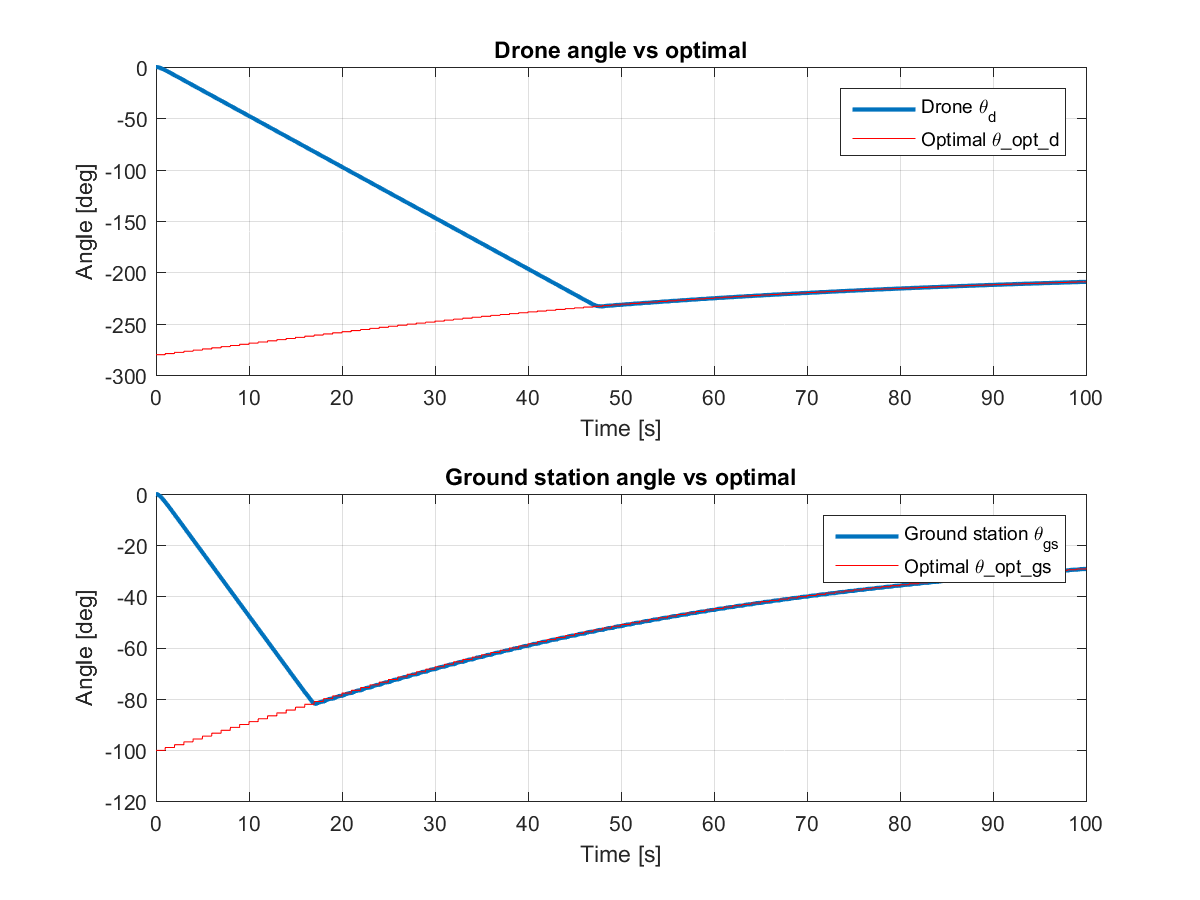
\includegraphics[scale=0.6]{figures/gs_angle_vs_optimal.png}
	\caption{GS angle vs optimal}
	\label{fig:gs_angle_vs_optimal}
\end{figure}

In this plot the angle is shown in degree to make it easier to understand. The blue line in both plots is respectively the UA and the GS antenna angle. They both start in 0 degree and have no initial starting point. Here it takes about 46 seconds for the UA's antenna to be at the optimal angle and in the other case it takes about 17 seconds for the GS antenna to turn to the optimal angle. But when they reached their optimal angle, the controller holds the antennas to the optimal angle. 
\newpage
